\documentclass[11pt,a4paper]{article}

\usepackage{fontspec}
\setmainfont{Latin Modern Roman}[Ligatures=TeX]
\setsansfont{Latin Modern Sans}[Ligatures=TeX]
\setmonofont{Latin Modern Mono}[Scale=0.95]
\usepackage[brazilian]{babel}
\usepackage[margin=2.5cm]{geometry}
\usepackage{microtype}
\usepackage{xcolor}
\usepackage{colortbl}
\usepackage{booktabs}
\usepackage{tabularx}
\usepackage{array}
\usepackage{float}
\usepackage{graphicx}
\usepackage{caption}
\usepackage{listings}
\usepackage{enumitem}
\usepackage{needspace}
\usepackage{fancyhdr}
\usepackage{titlesec}
\usepackage{amsmath}
\usepackage[hidelinks]{hyperref}

% Títulos em preto, discretos
\titleformat{\section}{\normalfont\large\bfseries}{\thesection}{0.6em}{}
\titleformat{\subsection}{\normalfont\normalsize\bfseries}{\thesubsection}{0.6em}{}
\titlespacing*{\section}{0pt}{1.4ex plus .4ex}{0.8ex}
\titlespacing*{\subsection}{0pt}{1.2ex plus .3ex}{0.6ex}

% Legendas: "Figura 1 — texto" e "Tabela 1 — texto"
\DeclareCaptionLabelSeparator{emdash}{ --- }
\captionsetup{labelsep=emdash,font=small,labelfont=bf,justification=raggedright,singlelinecheck=false}

\setlength{\parindent}{1.2em}
\emergencystretch=2em
\setlength{\parskip}{0.2em}
\renewcommand{\arraystretch}{1.15}

\pagestyle{fancy}
\fancyhf{}
\renewcommand{\headrulewidth}{0pt}
\fancyfoot[C]{\small\thepage}

\newcommand{\cab}[1]{\rowcolor{gray!22}#1}
\newcolumntype{Y}{>{\raggedright\arraybackslash}X}

\lstset{basicstyle=\ttfamily\footnotesize,breaklines=true,breakatwhitespace=false,
  columns=fullflexible,keepspaces=true,frame=single,rulecolor=\color{gray!60},
  xleftmargin=0.3em,xrightmargin=0.3em,aboveskip=0.6em,belowskip=0.4em,
  postbreak=\mbox{\textcolor{gray}{$\hookrightarrow$}\space}}

\begin{document}

\begin{center}
  {\LARGE\bfseries Relatório do Projeto 1}\\[0.3em]
  {\large\bfseries Busca e Organização de Dados}\\[0.3em]
  SCC0202 --- Algoritmos e Estruturas de Dados I
\end{center}

\noindent\textbf{Integrantes:} \\[0.3em]
\begin{tabular}{r @{ -- } l}
    17881457 & Bernardo Schramm Schutz Machado \\
    17899853 & João Pedro Cremasco Luiz \\
    15580336 & Thomas Riki Hashima
\end{tabular}

\vspace{0.8em} % Adiciona um espaçamento vertical adequado antes das partes

\noindent\textbf{Parte 1:} registros de aproximação de asteroides (\texttt{asteroid\_dataset\_20251019.csv}, 89.227 registros). \\
\textbf{Parte 2:} registros de jogos publicados na Steam (\texttt{games.csv}, 125.855 registros). \\
\textbf{Ambiente:} Linux x86\_64, Intel Core i5-10210U (4 núcleos, 8 threads, 15~GiB de RAM), GCC com \texttt{-std=c99 -Wall -Wextra -pedantic}. O executável \texttt{trabalho} é gerado por \texttt{make}.

%------------------------------------------------------------------
\section{Organização do código}

O programa lê um CSV, guarda cada linha como um ITEM na estrutura escolhida por \texttt{--base}, percorre essa estrutura aplicando a consulta, insere os itens aceitos na estrutura escolhida por \texttt{--result} e exporta até \texttt{top-k} registros. O fluxo é: leitor $\rightarrow$ ITEM $\rightarrow$ base $\rightarrow$ busca com a consulta $\rightarrow$ resultado $\rightarrow$ exportação $\rightarrow$ CSV.

\begin{table}[!htbp]
\centering
\caption{Módulos do programa e suas responsabilidades.}
\small
\begin{tabularx}{\textwidth}{@{}l Y@{}}
\toprule
\cab{\textbf{Módulo} & \textbf{Responsabilidade}} \\
\midrule
\texttt{src/\allowbreak{}item.c} & ITEM: conjunto de pares nome da coluna/valor em texto, independente do domínio. ITEM\_STORE: dono de todos os itens criados. \\
\texttt{src/\allowbreak{}reader.c} & Lê o cabeçalho, detecta o delimitador (vírgula, ponto e vírgula ou tabulação), trata campos entre aspas e vazios e cria os itens. É o único módulo específico de cada dataset (\texttt{--reader nasa}, \texttt{--reader games}). \\
\texttt{src/\allowbreak{}query.c} & Interpreta \texttt{FILTER}, \texttt{SIM}, \texttt{ACCEPT}, \texttt{ORDER}, \texttt{GROUP} e \texttt{CROSS}; decide se um item é aceito e calcula a similaridade. \\
\texttt{src/\allowbreak{}collection.c} & Interface comum às oito estruturas (criar, inserir, percorrer e destruir), com um \texttt{switch} sobre o tipo escolhido. \\
\texttt{src/\allowbreak{}export.c} & Escreve o CSV na ordem e no delimitador da entrada; em jogos, usa o cabeçalho corrigido para separar \texttt{Discount} e \texttt{DLC count}. \\
\texttt{src/\allowbreak{}main.c} & Argumentos, medição de tempo, orquestração e saída padrão. \\
\texttt{data\_\allowbreak{}structures/\allowbreak{}} & Oito TADs, um por arquivo, cada um com o seu nó ou vetor. \\
\bottomrule
\end{tabularx}
\end{table}

Os itens são guardados como texto e convertidos para número apenas quando uma consulta pede (\texttt{strtod}). Assim, valores ausentes não interrompem a leitura e o arquivo de saída reproduz o valor original.

%------------------------------------------------------------------
\section{Estruturas de dados}

Todas as estruturas foram implementadas pelo grupo, sem contêineres de bibliotecas externas. Elas não conhecem o conteúdo dos itens: guardam ponteiros genéricos, e o módulo \texttt{collection} converte para ITEM em um único ponto.

\begin{table}[!htbp]
\centering
\caption{Estruturas implementadas e o que diferencia cada uma.}
\footnotesize
\begin{tabularx}{\textwidth}{@{}l l Y Y@{}}
\toprule
\cab{\textbf{Estrutura} & \textbf{Argumento} & \textbf{Implementação} & \textbf{O que a diferencia}} \\
\midrule
Pilha & \texttt{stack} & vetor redimensionável & Inserção e remoção no topo; percurso do topo para a base. \\
Fila & \texttt{queue} & nós encadeados & Inserção no fim, remoção no início; percurso da frente para o fim. \\
Lista sequencial & \texttt{array\_\allowbreak{}list} & vetor redimensionável & Acesso por índice; a remoção desloca elementos. \\
Lista encadeada & \texttt{linked\_\allowbreak{}list} & nós duplamente encadeados, ponteiros para o primeiro e o último & Inserção no fim em tempo constante; remoção em qualquer posição. \\
Lista com cabeça & \texttt{sentinel\_\allowbreak{}list} & encadeada com sentinela real & O sentinela não representa registro; inserção, busca, remoção e percurso partem dele. \\
Lista ordenada & \texttt{ordered\_\allowbreak{}list} & vetor mantido em ordem & A posição é localizada por busca binária e o elemento é inserido já na ordem de \texttt{ORDER}, sem ordenar ao final. \\
Lista generalizada & \texttt{generalized\_\allowbreak{}list} & átomos e sublistas & \texttt{GROUP} cria grupos e subgrupos (por exemplo, categoria e depois ano); o percurso é em profundidade e visita apenas os itens. \\
Lista cruzada & \texttt{crossed\_\allowbreak{}list} & nós esparsos por par de chaves, ligados nas dimensões & A coleção guarda em cada célula os itens que compartilham o par de valores de \texttt{CROSS}. \\
\bottomrule
\end{tabularx}
\end{table}

Os nomes do enunciado (\texttt{pilha}, \texttt{fila}, \texttt{lista\_\allowbreak{}seq}, \texttt{lista\_\allowbreak{}enc}, \texttt{lista\_\allowbreak{}cabeca}, \texttt{lista\_\allowbreak{}ord}, \texttt{lista\_\allowbreak{}gen}, \texttt{lista\_\allowbreak{}cruz}) também são aceitos.

%------------------------------------------------------------------
\section{Consultas e exemplos de execução}\label{sec:exemplos}

A consulta é um arquivo texto com campos separados por \texttt{\textbar{}\allowbreak{}}. \texttt{FILTER} define condições obrigatórias (\texttt{==}, \texttt{!=}, \texttt{<}, \texttt{<=}, \texttt{>}, \texttt{>=}; numéricas quando os dois valores são números). \texttt{SIM} define um critério de similaridade
\[
  s(x,q,t)=\max\!\left(0,\;1-\frac{|x-q|}{t}\right),
\]
e a similaridade total é a média ponderada dos critérios. \texttt{ACCEPT} define o limiar mínimo. \texttt{ORDER}, \texttt{GROUP} e \texttt{CROSS} configuram a lista ordenada, a generalizada e a cruzada.

\subsection{Parte 1 --- Asteroides}

\Needspace{10\baselineskip}
\paragraph{Exemplo 1 --- filtro e similaridade.} Consulta \texttt{queries/\allowbreak{}asteroids\_\allowbreak{}by\_\allowbreak{}risk.txt}:
\begin{lstlisting}
FILTER|distance_au|<=|0.08
SIM|velocity_km_s|15.0|10.0|1.0
SIM|risk_score|0.70|0.30|2.0
ACCEPT|0.60
\end{lstlisting}
\begin{lstlisting}
./trabalho --reader nasa --input asteroid_dataset_20251019.csv --base linked_list --result array_list --query queries/asteroids_by_risk.txt --output resultados/asteroids_by_risk.csv --top-k 100 --limit 10000
\end{lstlisting}

\Needspace{10\baselineskip}
\paragraph{Exemplo 2 --- resultado ordenado.} Consulta \texttt{queries/\allowbreak{}asteroids\_\allowbreak{}ordered.txt}:
\begin{lstlisting}
FILTER|distance_au|<=|0.08
ORDER|risk_score|DESC
\end{lstlisting}
\begin{lstlisting}
./trabalho --reader nasa --input asteroid_dataset_20251019.csv --base queue --result ordered_list --query queries/asteroids_ordered.txt --output resultados/asteroids_ordered.csv --top-k 50 --limit 10000
\end{lstlisting}

\Needspace{10\baselineskip}
\paragraph{Exemplo 3 --- agrupamento e índice cruzado.} Consulta \texttt{queries/\allowbreak{}asteroids\_\allowbreak{}group\_\allowbreak{}cross.txt}:
\begin{lstlisting}
FILTER|distance_au|<=|0.1
GROUP|threat_category|year
CROSS|threat_category|year
\end{lstlisting}
\begin{lstlisting}
./trabalho --reader nasa --input asteroid_dataset_20251019.csv --base generalized_list --result crossed_list --query queries/asteroids_group_cross.txt --output resultados/asteroids_group_cross.csv --top-k 100 --limit 20000
\end{lstlisting}

\subsection{Parte 2 --- Jogos}

Os mesmos TADs são reutilizados, e apenas o leitor muda (\texttt{--reader games}). Esse leitor separa os nomes \texttt{Discount} e \texttt{DLC count}, que aparecem unidos no cabeçalho do arquivo fornecido.

\Needspace{10\baselineskip}
\paragraph{Exemplo 4 --- agrupamento por gênero e idade mínima.} Consulta \texttt{queries/\allowbreak{}games\_\allowbreak{}by\_\allowbreak{}genre.txt}:
\begin{lstlisting}
FILTER|Windows|==|true
FILTER|Price|>=|1
FILTER|Price|<=|100
SIM|Peak CCU|500|1000|1
ACCEPT|0.4
GROUP|Genres|Required age
\end{lstlisting}
\begin{lstlisting}
./trabalho --reader games --input games.csv --base linked_list --result generalized_list --query queries/games_by_genre.txt --output resultados/games_by_genre.csv --top-k 100 --limit 10000
\end{lstlisting}

\Needspace{10\baselineskip}
\paragraph{Exemplo 5 --- índice cruzado.} Consulta \texttt{queries/\allowbreak{}popular\_\allowbreak{}games\_\allowbreak{}by\_\allowbreak{}genre.txt}:
\begin{lstlisting}
FILTER|Peak CCU|>=|1000
FILTER|Windows|==|true
CROSS|Genres|Windows
\end{lstlisting}
\begin{lstlisting}
./trabalho --reader games --input games.csv --base array_list --result crossed_list --query queries/popular_games_by_genre.txt --output resultados/popular_games_by_genre.csv --top-k 100 --limit 10000
\end{lstlisting}

\Needspace{10\baselineskip}
\paragraph{Exemplo 6 --- outra combinação de TADs.} Consulta \texttt{queries/\allowbreak{}popular\_\allowbreak{}games\_\allowbreak{}ordered.txt}:
\begin{lstlisting}
FILTER|Windows|==|true
FILTER|Peak CCU|>=|1000
ORDER|Peak CCU|DESC
\end{lstlisting}
\begin{lstlisting}
./trabalho --reader games --input games.csv --base array_list --result ordered_list --query queries/popular_games_ordered.txt --output resultados/popular_games_ordered.csv --top-k 100 --limit 10000
\end{lstlisting}

\subsection{Resultados dos seis exemplos}

Os seis exemplos foram reexecutados três vezes nesta auditoria; as medições individuais estão em \texttt{resultados/examples\_raw.csv}. Os arquivos de asteroides mantêm o cabeçalho original. O arquivo de jogos tem o nome \texttt{DiscountDLC count} unido no cabeçalho, embora os registros tenham duas colunas; o leitor o separa em \texttt{Discount} e \texttt{DLC count}, e a exportação usa esses nomes corrigidos. A ordem das colunas e o delimitador são mantidos.

\begin{table}[!htbp]
\centering
\caption{Resultados dos exemplos de execução (médias de três execuções, tempos em ms).}
\footnotesize
\setlength{\tabcolsep}{4pt}
\begin{tabular}{@{}r p{4.3cm} r r r r r r r@{}}
\toprule
\cab{\textbf{Ex.} & \textbf{Base $\rightarrow$ resultado} & \textbf{Lidos} & \textbf{Enc.} & \textbf{Exp.} & \textbf{Carga} & \textbf{Busca} & \textbf{Ins. res.} & \textbf{Escrita}} \\
\midrule
1 & \texttt{linked\_\allowbreak{}list}$\rightarrow$\texttt{array\_\allowbreak{}list} & 10.000 & 93 & 93 & 90,331 & 15,793 & 0,010 & 1,037 \\
2 & \texttt{queue}$\rightarrow$\texttt{ordered\_\allowbreak{}list} & 10.000 & 5.501 & 50 & 94,582 & 20,983 & 140,346 & 0,620 \\
3 & \texttt{generalized\_\allowbreak{}list}$\rightarrow$\texttt{crossed\_\allowbreak{}list} & 20.000 & 12.919 & 100 & 214,005 & 45,261 & 13,927 & 1,201 \\
4 & \texttt{linked\_\allowbreak{}list}$\rightarrow$\texttt{generalized\_\allowbreak{}list} & 10.000 & 6.145 & 100 & 908,436 & 35,567 & 24,307 & 7,651 \\
5 & \texttt{array\_\allowbreak{}list}$\rightarrow$\texttt{crossed\_\allowbreak{}list} & 10.000 & 43 & 43 & 900,082 & 7,488 & 0,124 & 4,923 \\
6 & \texttt{array\_\allowbreak{}list}$\rightarrow$\texttt{ordered\_\allowbreak{}list} & 10.000 & 43 & 43 & 910,608 & 15,011 & 0,147 & 4,274 \\
\bottomrule
\end{tabular}
\end{table}

%------------------------------------------------------------------
\section{Memória}

Os itens pertencem ao ITEM\_STORE. As estruturas guardam ponteiros emprestados e liberam apenas o que alocam para se organizar (nós, vetores e índices). Assim, o mesmo item pode estar ao mesmo tempo na base, no resultado e nos dois índices da lista cruzada, sem cópia e sem liberação dupla. No fim da execução, as coleções são destruídas primeiro e o store por último.

Os seis exemplos executados com AddressSanitizer e UndefinedBehaviorSanitizer terminaram sem erros reportados, com a detecção de vazamentos do LeakSanitizer desativada por incompatibilidade do ambiente. Valgrind não encontrou erros nem vazamentos nos exemplos 1, 3, 4 e 5, nem na suíte dos TADs.

%------------------------------------------------------------------
\section{Complexidade assintótica}

Seja $n$ o número de itens armazenados, $k$ o número de registros exportados, $p$ o número de campos por item, $g$ o número de grupos, $s$ o de subgrupos examinados, $m$ o de itens no subgrupo, $r$ e $c$ o número de chaves distintas dos índices da lista cruzada, $h$ os itens no bucket da célula e $d_r$ e $d_c$ os graus da linha e da coluna percorridas.

\begin{table}[!htbp]
\centering
\caption{Complexidade das operações realmente usadas pelo programa.}
\small
\begin{tabularx}{\textwidth}{@{}l Y Y Y@{}}
\toprule
\cab{\textbf{Estrutura} & \textbf{Inserção} & \textbf{Busca / percurso} & \textbf{Remoção}} \\
\midrule
Pilha & $O(1)$ amortizado; $O(n)$ ao redimensionar & $O(n)$ & $O(1)$ no topo; localizar item arbitrário $O(n)$ \\
Fila & $O(1)$ & $O(n)$ & $O(1)$ na frente; localizar item arbitrário $O(n)$ \\
Lista sequencial & $O(1)$ amortizado no fim & $O(n)$ & $O(n)$, pois busca e desloca \\
Lista encadeada & $O(1)$ no fim (ponteiro final) & $O(n)$ & $O(n)$ para localizar; $O(1)$ para religar \\
Lista com cabeça & $O(1)$ no fim & $O(n)$ & $O(n)$ para localizar; $O(1)$ para religar \\
Lista ordenada & $O(n)$: busca binária $O(\log n)$ mais deslocamento $O(n)$ & $O(\log n)$ por chave; $O(n)$ para percorrer & $O(n)$ \\
Lista generalizada & $O(g+s)$ para achar ou criar grupo e subgrupo; $O(1)$ para anexar & $O(n)$ & $O(g+s+m)$ no pior caso \\
Lista cruzada & $O(r+c+d_r+d_c)$ para célula nova; $O(r+c)$ para anexar em célula existente & $O(n)$ total; $O(d_r)$ ou $O(d_c)$ por linha ou coluna & $O(r+c+h)$ para localizar chaves e item no bucket \\
\bottomrule
\end{tabularx}
\end{table}

Carregar $n$ itens custa $O(n)$ amortizado em pilha, fila e listas simples. Na lista ordenada pode custar $O(n^2)$ pelos deslocamentos, e na generalizada e na cruzada depende da quantidade de chaves distintas e dos graus. A busca da consulta percorre os $n$ itens da base independentemente da estrutura. Como \texttt{item\_get} percorre linearmente os $p$ campos do item, o custo é $O(n(f+q)p)$ para $f$ filtros e $q$ critérios \texttt{SIM}, mais a inserção dos aceitos e a gravação do campo \texttt{similarity}, que acrescenta um campo ao item. A exportação custa $O(kp^2)$, pois cada uma das $p$ colunas é procurada no item, mais a escrita dos caracteres.

%------------------------------------------------------------------
\section{Avaliação experimental}

\subsection{Protocolo}

\begin{itemize}[nosep]
  \item Base \texttt{linked\_\allowbreak{}list} e resultado \texttt{array\_\allowbreak{}list} nos dois datasets; foram usadas as consultas de benchmark de asteroides e jogos.
  \item Seis pares de \texttt{--limit} e \texttt{--top-k}: (1.000, 10), (5.000, 50), (10.000, 100), (25.000, 500), (50.000, 1.000) e (0, 0), em que zero significa toda a base e todos os resultados.
  \item Cada configuração teve uma execução de aquecimento, descartada, e três execuções medidas. As tabelas mostram a média aritmética e o desvio padrão amostral ($\pm$). As 36 medições individuais estão em \texttt{resultados/\allowbreak{}benchmark\_\allowbreak{}raw.csv}.
  \item A coluna $N$ é o número de registros lidos (\texttt{INPUT\_\allowbreak{}RECORDS}).
\end{itemize}

\subsection{Metodologia de medição}\label{sec:met}

Os tempos são medidos dentro do próprio programa com \texttt{clock()} de \texttt{time.h} (C99), que devolve o tempo de CPU do processo, usuário mais sistema, em ticks de $1/\texttt{CLOCKS\_PER\_SEC}$ (1~µs no Linux), convertido para milissegundos. Cada fase é delimitada por duas leituras do relógio. Como o relógio mede CPU e não tempo decorrido, esperas por disco não entram nas medições, e os valores de carga e de saída não equivalem à latência percebida pelo usuário.

A busca e a inserção no resultado são feitas em duas passadas. Na primeira, \texttt{collection\_visit} avalia os critérios de cada item, grava o campo \texttt{similarity} e guarda o ponteiro dos itens aceitos em um vetor. Na segunda, um laço insere todos eles na estrutura do resultado, com um único par de chamadas a \texttt{clock()} ao redor do laço inteiro. Assim, a busca não inclui a inserção, e o relógio não é lido uma vez por item. Não entram nas medições a abertura do arquivo de entrada, a leitura da consulta, a criação e a destruição das estruturas e a inicialização do processo, e por isso a coluna Total é a soma das quatro fases, e não o tempo de parede do programa.

A medição por item faria duas leituras de \texttt{clock()} para cada inserção e repetiria esse custo muitas vezes. Por isso, o programa mede o laço inteiro em bloco.

A máquina não estava isolada. No momento da coleta, o load average era 6,64, 6,26 e 6,00; a frequência reportada estava em 57% do máximo nominal. Essa observação pontual não representa a carga durante toda a série. As Tabelas~\ref{tab:ast} e~\ref{tab:jogos} usam as abreviações do glossário abaixo.

\begin{table}[!htbp]
\centering
\caption{Glossário das colunas das tabelas de tempos.}
\label{tab:glossario}
\small
\begin{tabularx}{\textwidth}{@{}l l Y@{}}
\toprule
\cab{\textbf{Coluna} & \textbf{Saída do programa} & \textbf{O que mede}} \\
\midrule
$N$ & \texttt{INPUT\_RECORDS} & Registros lidos da entrada, limitados por \texttt{--limit} (0 lê toda a base). \\
$k$ & \texttt{OUTPUT\_RECORDS} & Máximo de registros exportados, definido por \texttt{--top-k} (0 exporta todos). \\
Carga & \texttt{LOAD\_MS} & Laço que lê cada registro do CSV (leitura, separação de campos e criação do ITEM) e o insere na estrutura da base. \\
Busca & \texttt{SEARCH\_MS} & Percurso da base com \texttt{collection\_visit}, avaliando \texttt{FILTER}, \texttt{SIM} e \texttt{ACCEPT} em cada item e guardando os aceitos em um vetor (primeira passada). \\
Ins. res. & \texttt{RESULT\_INSERT\_MS} & Laço de \texttt{collection\_insert} que passa os itens aceitos para a estrutura do resultado (segunda passada), medido em bloco. \\
Saída (Escrita) & \texttt{WRITE\_MS} & \texttt{export\_write}: abrir o arquivo, escrever o cabeçalho, percorrer o resultado até $k$ e gravar as linhas. \\
Total & --- & Soma de Carga, Busca, Ins. res. e Saída. \\
Enc. / exp. & \texttt{MATCHED\_RECORDS} / \texttt{OUTPUT\_RECORDS} & Registros aceitos pela consulta e registros exportados. \\
\bottomrule
\end{tabularx}
\end{table}

\subsection{Resultados}

\begin{table}[!htbp]
\centering
\caption{Asteroides (89.227 registros no arquivo), \texttt{linked\_\allowbreak{}list}\,$\rightarrow$\allowbreak\,\texttt{array\_\allowbreak{}list}. Média $\pm$ desvio padrão, em ms.}
\label{tab:ast}
\small
\setlength{\tabcolsep}{4pt}
\resizebox{\textwidth}{!}{%
\begin{tabular}{@{}r r r r r r r r@{}}
\toprule
\cab{$\boldsymbol{N}$ & $\boldsymbol{k}$ & \textbf{Carga} & \textbf{Busca} & \textbf{Ins. res.} & \textbf{Saída} & \textbf{Total} & \textbf{Enc. / exp.}} \\
\midrule
1.000 & 10 & 9,915 $\pm$ 1,144 & 2,488 $\pm$ 0,330 & 0,024 $\pm$ 0,001 & 0,337 $\pm$ 0,094 & 12,764 $\pm$ 1,102 & 649 / 10 \\
5.000 & 50 & 45,734 $\pm$ 1,525 & 10,906 $\pm$ 1,447 & 0,093 $\pm$ 0,024 & 0,696 $\pm$ 0,028 & 57,429 $\pm$ 1,598 & 3.195 / 50 \\
10.000 & 100 & 93,834 $\pm$ 2,991 & 21,003 $\pm$ 2,083 & 0,225 $\pm$ 0,093 & 1,128 $\pm$ 0,108 & 116,190 $\pm$ 3,057 & 6.323 / 100 \\
25.000 & 500 & 259,943 $\pm$ 10,395 & 58,729 $\pm$ 3,694 & 0,507 $\pm$ 0,090 & 4,625 $\pm$ 0,597 & 323,805 $\pm$ 9,731 & 15.249 / 500 \\
50.000 & 1.000 & 510,761 $\pm$ 8,330 & 101,930 $\pm$ 9,109 & 0,746 $\pm$ 0,247 & 8,911 $\pm$ 1,121 & 622,348 $\pm$ 13,754 & 24.012 / 1.000 \\
89.227 (toda) & todos & 970,935 $\pm$ 13,388 & 187,741 $\pm$ 15,744 & 1,100 $\pm$ 0,166 & 332,816 $\pm$ 18,368 & 1.492,593 $\pm$ 36,418 & 39.380 / 39.380 \\
\bottomrule
\end{tabular}}
\end{table}

\begin{table}[!htbp]
\centering
\caption{Jogos (125.855 registros no arquivo), \texttt{linked\_\allowbreak{}list}\,$\rightarrow$\allowbreak\,\texttt{array\_\allowbreak{}list}. Média $\pm$ desvio padrão, em ms.}
\label{tab:jogos}
\small
\setlength{\tabcolsep}{4pt}
\resizebox{\textwidth}{!}{%
\begin{tabular}{@{}r r r r r r r r@{}}
\toprule
\cab{$\boldsymbol{N}$ & $\boldsymbol{k}$ & \textbf{Carga} & \textbf{Busca} & \textbf{Ins. res.} & \textbf{Saída} & \textbf{Total} & \textbf{Enc. / exp.}} \\
\midrule
1.000 & 10 & 93,164 $\pm$ 6,064 & 3,582 $\pm$ 0,335 & 0,037 $\pm$ 0,003 & 0,817 $\pm$ 0,202 & 97,601 $\pm$ 6,179 & 1.000 / 10 \\
5.000 & 50 & 449,742 $\pm$ 26,568 & 16,095 $\pm$ 3,451 & 0,140 $\pm$ 0,011 & 3,270 $\pm$ 0,857 & 469,247 $\pm$ 29,737 & 4.998 / 50 \\
10.000 & 100 & 879,470 $\pm$ 19,230 & 30,877 $\pm$ 1,333 & 0,297 $\pm$ 0,057 & 6,746 $\pm$ 0,558 & 917,390 $\pm$ 19,934 & 9.996 / 100 \\
25.000 & 500 & 2.218,394 $\pm$ 18,373 & 78,598 $\pm$ 7,154 & 0,818 $\pm$ 0,096 & 30,340 $\pm$ 3,386 & 2.328,149 $\pm$ 25,470 & 24.989 / 500 \\
50.000 & 1.000 & 4.602,054 $\pm$ 165,089 & 184,245 $\pm$ 7,737 & 1,835 $\pm$ 0,098 & 65,157 $\pm$ 6,400 & 4.853,291 $\pm$ 156,493 & 49.978 / 1.000 \\
125.855 (toda) & todos & 11.657,033 $\pm$ 123,182 & 413,325 $\pm$ 45,218 & 3,807 $\pm$ 0,397 & 7.962,563 $\pm$ 317,230 & 20.036,727 $\pm$ 474,308 & 125.811 / 125.811 \\
\bottomrule
\end{tabular}}
\end{table}

\begin{figure}[!htbp]
\centering
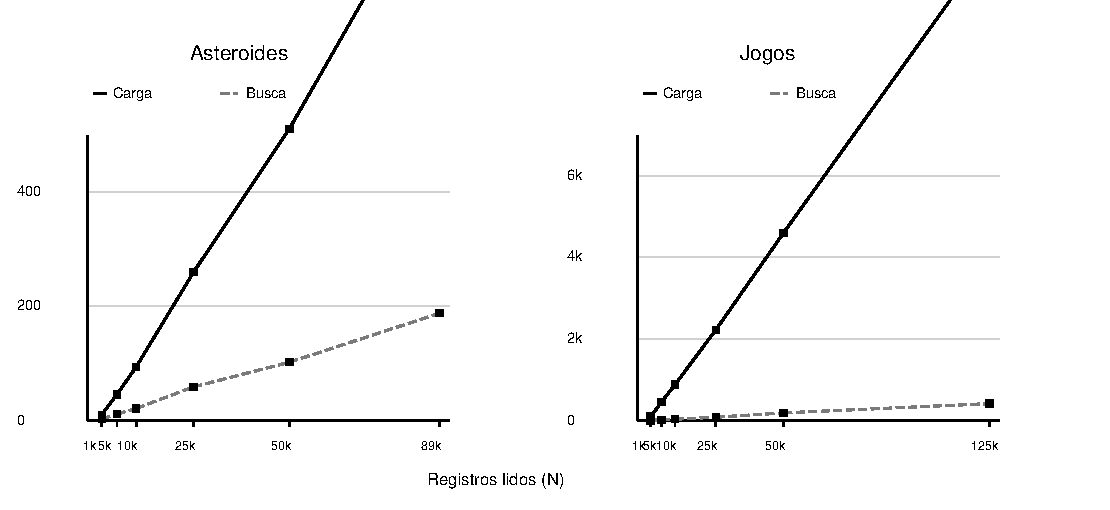
\includegraphics[width=\textwidth]{docs/fig/fig_carga_busca.pdf}
\caption{Tempo médio de carga e de busca em função do número de registros lidos, para os dois datasets (valores das Tabelas~\ref{tab:ast} e~\ref{tab:jogos}).}
\label{fig:carga-busca}
\end{figure}

\subsection{Custo por registro}

Para comparar com o crescimento esperado, a Tabela~\ref{tab:custo-registro} divide os tempos médios pelo número de registros lidos (carga e busca) ou exportados (saída), em microssegundos.

\begin{table}[!htbp]
\centering
\caption{Custo por registro (µs), calculado com as médias não arredondadas de \texttt{benchmark\_raw.csv}.}
\label{tab:custo-registro}
\small
\setlength{\tabcolsep}{5pt}
\begin{tabular}{@{}l r r r r r r@{}}
\toprule
\cab{\textbf{Dataset} & $\boldsymbol{N}$ & \textbf{Carga / lido} & \textbf{Busca / lido} & \textbf{Ins. / aceito} & $\boldsymbol{k}$ & \textbf{Saída / exp.}} \\
\midrule
Asteroides & 1.000 & 9,92 & 2,49 & 0,04 & 10 & 33,70 \\
Asteroides & 25.000 & 10,40 & 2,35 & 0,03 & 500 & 9,25 \\
Asteroides & 89.227 & 10,88 & 2,10 & 0,03 & 39.380 & 8,45 \\
Jogos & 1.000 & 93,16 & 3,58 & 0,04 & 10 & 81,70 \\
Jogos & 25.000 & 88,74 & 3,14 & 0,03 & 500 & 60,68 \\
Jogos & 125.855 & 92,62 & 3,28 & 0,03 & 125.811 & 63,29 \\
\bottomrule
\end{tabular}
\end{table}

\subsection{Custo de inserir no resultado, por estrutura}

A Tabela~\ref{tab:insercao} divide o tempo de inserção pelo número de itens aceitos.

\begin{table}[!htbp]
\centering
\caption{Custo de inserção no resultado por estrutura, nos exemplos da Seção~\ref{sec:exemplos}.}
\label{tab:insercao}
\small
\begin{tabular}{@{}r l r r r@{}}
\toprule
\cab{\textbf{Ex.} & \textbf{Estrutura do resultado} & \textbf{Itens inseridos} & \textbf{Ins. res. (ms)} & \textbf{Por item (µs)}} \\
\midrule
1 & \texttt{array\_\allowbreak{}list} & 93 & 0,010 & 0,10 \\
2 & \texttt{ordered\_\allowbreak{}list} & 5.501 & 140,346 & 25,51 \\
3 & \texttt{crossed\_\allowbreak{}list} & 12.919 & 13,927 & 1,08 \\
4 & \texttt{generalized\_\allowbreak{}list} & 6.145 & 24,307 & 3,96 \\
5 & \texttt{crossed\_\allowbreak{}list} & 43 & 0,124 & 2,88 \\
6 & \texttt{ordered\_\allowbreak{}list} & 43 & 0,147 & 3,41 \\
\bottomrule
\end{tabular}
\end{table}

\begin{figure}[!htbp]
\centering
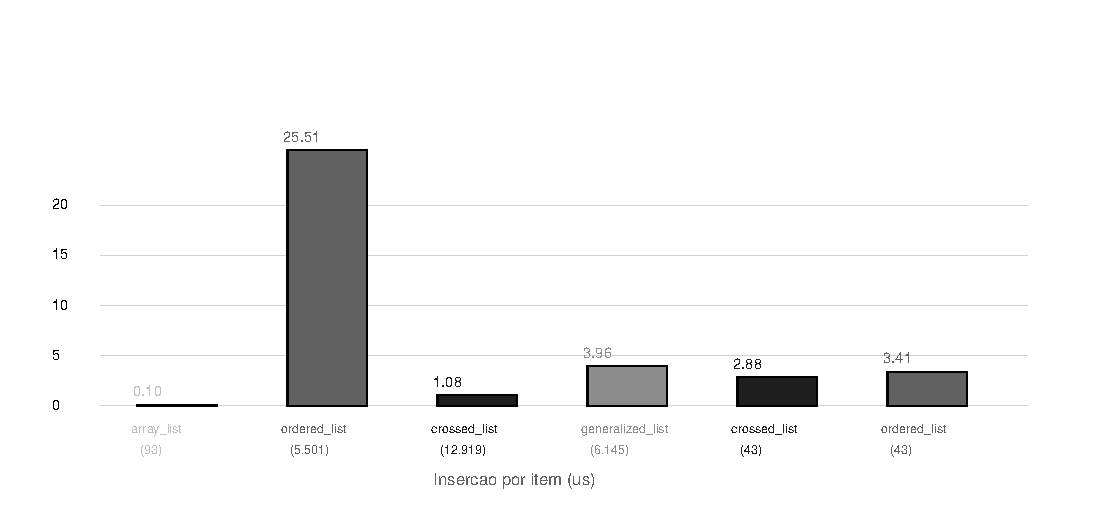
\includegraphics[width=\textwidth]{docs/fig/fig_insercao.pdf}
\caption{Custo de inserção por item nos seis exemplos, com a quantidade de itens entre parênteses.}
\label{fig:insercao}
\end{figure}

\subsection{Discussão}

\paragraph{Carga e busca.} Ambas crescem com $N$, conforme o percurso linear da base. Na tabela selecionada, a carga por registro ficou entre 9,92 e 10,88~µs em asteroides e entre 88,74 e 93,16~µs em jogos; a busca ficou entre 2,10 e 2,49~µs em asteroides e entre 3,14 e 3,58~µs em jogos. Na base completa, o desvio padrão da carga foi 13,388~ms em asteroides e 123,182~ms em jogos. Para asteroides com $N=50.000$, as cargas medidas foram 501,255, 514,242 e 516,786~ms.

\paragraph{Inserção no resultado.} Com \texttt{array\_\allowbreak{}list}, medida em bloco, a inserção média na base completa foi 1,100~ms para 39.380 itens de asteroides e 3,807~ms para 125.811 itens de jogos.

\paragraph{Composição do total e saída.} Na base completa, carga, busca, inserção e escrita representam 65,05\%, 12,58\%, 0,07\% e 22,30\% para asteroides, e 58,18\%, 2,06\%, 0,02\% e 39,74\% para jogos. Para $k=10$, o custo de saída é 33,70~µs por registro em asteroides e 81,70~µs em jogos; esse valor inclui abrir o arquivo e gravar o cabeçalho. O custo é $O(kp^2)$, pois cada coluna procura seu valor com \texttt{item\_get}.

\paragraph{Estruturas avançadas.} A Tabela~\ref{tab:insercao} e a Figura~\ref{fig:insercao} comparam os seis exemplos medidos. O custo por item variou de 0,10 a 25,51~µs. São casos diferentes e a comparação é qualitativa.

\paragraph{Limitações.} Os experimentos controlados mantiveram base e resultado fixos (\texttt{linked\_\allowbreak{}list}$\rightarrow$\allowbreak{}\texttt{array\_\allowbreak{}list}). As estruturas avançadas aparecem apenas nos seis exemplos, que diferem em consulta, dataset e tamanho; a comparação da Tabela~\ref{tab:insercao} é, portanto, qualitativa e não substitui um fatorial de benchmark. Cada medição se baseia em apenas três execuções, e a máquina não estava isolada (Seção~\ref{sec:met}). Cada configuração teve um aquecimento seguido de três medidas; o aquecimento não é gravado no CSV. Como o relógio mede CPU, esperas de disco não aparecem. Todas as medições foram feitas em uma única máquina.

%------------------------------------------------------------------
\section{Conclusão}

As oito estruturas estão disponíveis pela mesma interface de coleção. A série de benchmark foi repetida para os dois datasets, com aquecimento e três medidas por configuração. Na base completa, a carga domina o tempo total, enquanto a escrita também tem peso relevante, especialmente em jogos.

Nos seis exemplos, os custos de inserção por item variaram de 0,10 a 25,51~µs. A lista cruzada agrupa itens com as mesmas chaves em uma lista por célula. Os exemplos diferem em consulta, dataset e quantidade de itens, então a comparação é qualitativa.

\end{document}
